\documentclass[11pt, openany]{article}

\usepackage[T1]{fontenc}
\usepackage[utf8]{inputenc}
\usepackage[english, italian]{babel}
\usepackage{cancel}

\usepackage{hyperref}
\hypersetup{colorlinks=true,
	linkcolor=black,
	citecolor= black,
	filecolor=magenta,
	urlcolor=cyan,
}

\usepackage{geometry}
\geometry{
	a4paper,
	top=2.5cm,
	bottom=2cm,
	left=1.5cm,
	right=1.5cm,
	heightrounded,
	bindingoffset=5mm
}

\usepackage{amsmath}
\usepackage{amssymb}
\usepackage{amsthm}
\usepackage{tabularx}
\usepackage{booktabs}
\usepackage{caption}
\captionsetup{font = smaller}
\usepackage{enumitem}
\usepackage{blindtext}
\usepackage[x11names]{xcolor}
\usepackage{tcolorbox}
\usepackage{graphicx}
\usepackage{pdfpages}
\usepackage[export]{adjustbox}
\usepackage{cleveref}
\usepackage{multirow}



\theoremstyle{definition}
\newtheorem*{defn}{Definizione}
\newtheorem{exe}{Esercizio}[section]
\newtheorem{esem}{Esempio}[section]
\theoremstyle{plain}
\theoremstyle{remark}
\newtheorem*{warn}{ATTENZIONE}
\newtheorem*{svol}{Svolgimento}

\setcounter{secnumdepth}{-1}
\setcounter{tocdepth}{4}


\setlist[itemize]{nosep}
\usepackage{helvet}
\renewcommand{\familydefault}{\sfdefault}


\title{Relazione \\\textbf {Progetto A.A. 2022/2023 \\ ADAS made trivial: rappresentazione \underline{ispirata} alle
		interazioni in un sistema di guida autonoma}}
\author{Diciotti \hfill Matteo \\\\ 7072181 \and Manucci \hfill Agostino \\\\ 7084379 \and Montes Anacona \\ Àlvaro \\ 7117731}
\date{1 giugno 2023 - \today}

\begin{document}
	\maketitle
	\hrule
	\vspace{1cm}

	\part[Presentazione]{}
		\paragraph{Titolo}
			Progetto A.A. 2022/2023 – ADAS made trivial: rappresentazione \underline{ispirata} alle interazioni in un sistema di guida autonoma
		\paragraph{Autori}
			\footnotesize Lista degli autori ordinata per numero di matricola\\
			\normalsize
			\begin{tabularx}{\textwidth}[t]{p{4.5cm} p{3.5cm} p{2.5cm} r}
				\textbf{Matricola} 	& 	\textbf{Cognome} 	& 	\textbf{Nome} 	& \textbf{e-mail} 					\\\toprule
				7072181				&	Diciotti			&	Matteo			&	matteo.diciotti@stud.unifi.it	\\
				7084379				&	Mannucci			&	Agostino		&	agostino.mannucci@stud.unifi.it	\\
				7117731				&	Montes Anacona		&	Àlvaro			&	\dots
			\end{tabularx}

		\paragraph{Obbiettivo}
			Obiettivo del progetto è costruire un’architettura, estremamente stilizzata e rivisitata, per sistemi ADAS,
			descrivendo possibili interazioni e alcuni comportamenti tra componenti in scenari specifici.

	\part{Introduzione}
		\paragraph{Introduzione al progetto}
			Un \textit{\textbf{A}dvanced \textbf{D}river \textbf{A}ssistance \textbf{S}ystem} è un sistema composto da varie componenti che cooperano affinché un veicolo o un mezzo possano assistere un conducente nella guida e in alcuni contesti sostituirsi al guidatore stesso.\\
			Il progetto realizzato cerca di riprodurre fedelmente il sistema simulativo di un ADAS presentato nella richiesta\footnote{Per visionare la richiesta dell'elaborato riferirsi al documento Allegato\_1.pdf compreso nella cartella del progetto} dell'elaborato nella quale sono definite varie componenti suddivise in quattro gruppi: \textit{interfaccia}, \textit{attuatori}, \textit{sensori} e \textit{controllo}.\\
			La simulazione è resa effettiva dall'inserimento di stringhe rappresentanti le azioni che dovrebbero essere eseguite dalle varie componenti di un ADAS in dei file di log specifici per ogni componente. In particolare le componenti implementate sono nove, sette obbligatorie e due facoltative\footnote{Per conoscere quali elementi facoltativi sono stati implementati visionare la tabella~\ref{tab:facoltativi}}.\\
			I \textit{sensori}, attraverso l'acquisizione di dati da file predefiniti o da sorgenti casuali, simulano l'acquisizione di dati da parte di sensori reali e li inviano all'unica componente di controllo, la componente \textit{Central ECU}. Gli \textit{attuatori} ricevono messaggi dall'unità di controllo ed eseguono scritture nell'apposito file di log per simulare la messa in atto dell'attuazione del comando su di un attuatore reale. Infine la componente con cui si interfaccia l'esecutore del programma è la \textit{Human-Machine Interface} che simula l'interfaccia del guidatore attendendo comandi (in questo caso scritti su di un terminale) e mostrando i risultati e le conseguenze dei propri comandi (nel caso della simulazione saranno scritti su di un differente terminale tutti i comandi che l'unita di controllo centrale ha inviato alle varie componenti).

		\paragraph{Impostazione del lavoro}
			Al fine di realizzare un sistema che simulasse un ADAS sono state eseguite alcune fasi per il completamento del programma: l'analisi delle richieste, la strutturazione teorica dell'architettura del sistema, l'implementazione pratica, la verifica e revisione dell'elaborato.\\
			Ad una prima fase di studio delle richieste congiunta tra gli autori del progetto è immediatamente succeduta la fase di strutturazione dello stesso, anch'essa svolta unitamente tra i relatori, giungendo alla teorizzazione dell'architettura mostrata in figura~\ref{fig:gerarchia}. Sono stati quindi divisi i lavori per l'implementazione del programma tra i componenti del gruppo e uniti gli elaborati in un unico componimento comprensivo di makefile e file binari per l'esecuzione in modalità \textit{ARTIFICIALE} del programma. Sono state quindi eseguite ciclicamente le due fasi di verifica e di revisione: nella prima fase sono stati svolti test per verificare il corretto funzionamento dell'elaborato per entrambe le modalità e nella seconda fase sono state apportate le modifiche necessarie affinché il programma producesse i risultati attesi. Infine e` stata prodotta la presente relazione.
	\part{Specifiche}
		\paragraph{Caratteristiche HW e SW}
		Per l'implementazione sono stati utilizzati tre hardware differenti con tre sistemi operativi differenti:
		\begin{itemize}
			\item \textbf{ArchLinux}, vers. \dots, kernel linux \dots, architettura x86\_64
			\item \textbf{Manjaro}, vers, \dots,kernel linux \dots, architettura x86\_64
			\item \textbf{Ubuntu 20.04}, kernel linux \dots, architettura x86\_64
		\end{itemize}
		Il progetto è stato ideato avendo come obbiettivo un programma portatile che fosse preimpostato per eseguire su di un sistema \textbf{\underline{Ubuntu Linux 22.04}}.
		\paragraph{Istruzioni compilazione ed esecuzione}
		\paragraph{Elementi facoltativi}
			La tabella seguente mostra gli elementi facoltativi implementati seguiti da una breve descrizione dell'implementazione.
			\begin{tcolorbox}[width=\textwidth,colback={Cornsilk2}]
				\begin{tabularx}{\textwidth}{lXcX}
					\textbf{\#}	&	\textbf{Elemento facoltativo}	&	\textbf{Realizzato (SI/NO)}	&	\textbf{Descriizone dell'implementazione con indicazione del metodo/i principale/i} \\\toprule\vspace{.1cm}
					\multirow{8}*{1}	&	Ad ogni accelerazione, c’è una probabilità di $10^{-5}$ che l’acceleratore fallisca. In tal caso, il componente \textit{throttle control} invia un \underline{segnale} alla \textit{Central ECU} per evidenziare tale evento, e la Central ECU avvia la procedura di \textit{ARRESTO} & \multirow{8}*{SI} & \dots \\\vspace{0.1cm}
					\multirow{2}*{2}	&	Componente \textit{forward facing radar}	&	\multirow{2}*{SI}	&	\dots	\\\vspace{0.1cm}
					\multirow{5}*{3}	&	Quando si attiva l’interazione con park assist, la \textit{Central ECU} sospende (o rimuove) tutti i sensori e attuatori, tranne \textit{park assist} e \textit{surround view cameras}	&	\multirow{5}*{SI}	&	\dots	\\\vspace{0.1cm}
					\multirow{4}*{4}	&	Il componente \textit{park assist} non è generato all'avvio del sistema, ma creato dalla \textit{Central ECU} al bisogno	&	\multirow{4}*{SI}	&	\dots	\\\vspace{0.1cm}
					\multirow{5}*{5}	&	Se il componente \textit{surround view cameras} è implementato, \textit{park assist} trasmette a \textit{Central ECU} anche i byte ricevuti da \textit{surround view cameras}	&	\multirow{5}*{SI}	&	\dots	\\\vspace{0.1cm}
					\multirow{2}*{6}	&	Componente \textit{surround view cameras}	&	\multirow{2}*{SI}	&	\dots	\\\vspace{0.1cm}
					\multirow{7}*{7}	&	Il comando di \textit{PARCHEGGIO} potrebbe arrivare mentre i vari attuatori stanno eseguendo ulteriori comandi (accelerare o sterzare). I vari attuatori interrompono le loro azioni, per avviare le procedure di parcheggio	&	\multirow{7}*{SI}	&	\dots	\\
					\multirow{6}*{8}	&	Se la \textit{Central ECU }riceve il segnale di fallimento accelerazione da \textit{throttle control}, imposta la velocità a 0 e invia all'output della \textit{HMI} un messaggio di totale terminazione dell'esecuzione	&	\multirow{6}*{SI}	&	\dots
				\end{tabularx}
				\label{tab:facoltativi}
			\end{tcolorbox}

	\part{Descrizione architettura sistema}
		Nella sezione viene presentata l'architettura del progetto e le scelte implementative prese, cercando di descrivere i motivi che hanno portato alle singole decisioni prese.

		\paragraph{Implementazione componenti}
			\footnotesize Segue una tabella nella quale si mostrano quali sorgenti implementano le componenti
			\normalsize

			\begin{tcolorbox}[width=\textwidth,colback={Cornsilk2}]\label{tab:sorgenti}
				\begin{tabularx}{\textwidth}{p{8cm}  l}
					\textbf{Componente}			&	\textbf{Sorgente}	\\\toprule
					Human-Machine Interface 	& 	hmi-input.c			\\
												&	hmi-output.c		\\\midrule
					steer-by-wire				&	steer-by-wire.c		\\\midrule
					throttle control			&	throttle-control.c	\\\midrule
					brake-by-wire				&	brake-by-wire		\\\midrule
					front windshield camera		&	windshield-camera.c	\\\midrule
					forward facing radar		&	bytes-sensors.c		\\\midrule
					park assist					&	park-assist.c		\\\midrule
					surround view cameras		&	bytes.sensors.c		\\\midrule
					central ECU					&	central-ECU.c


				\end{tabularx}
			\end{tcolorbox}

		\paragraph{Gerarchia del programma}
			La gerarchia del progetto è stata ottenuta dalla richiesta cercando di massimizzare la semplicità.\\
			Questa rappresenta lo scheletro del progetto e definisce quindi il flusso di lavoro dello stesso. In particolare si può notare in figura~\ref{fig:gerarchia} che esistono due soli processi che inizializzano dei figli, ovvero l'unita di controllo centrale \textit{central-ECU}, che rappresenta anche il programma genitore di tutto il sistema, e \textit{park-assist}, che inizializza il suo unico figlio \textit{surround-view cameras}.\\
			È stato scelto di rendere l'unità di controllo genitore di tutto il sistema dato essere in collegamento con la quasi totalità dei processi agenti, cosicché il sistema fosse interamente inizializzato in un solo intervallo temporale da un unico processo.\\
			Infatti, nella \textit{central-ECU} vengono immediatamente inizializzati i pipe, dopodiché vengono eseguite varie \texttt{fork} per la creazione e la connessione in lettura/scrittura ai pipe degli attuatori, dei componenti della \textit{Human-Machine Interface} e i sensori \textit{front windshield camera} e \textit{forward facing radar}. L'unico componente figlio della \textit{central-ECU} non immediatamente inizializzato rimane \textit{park-assist}\footnote{La decisione di non inizializzare il componente immediatamente deriva dalla richiesta, ovvero dall'elemento facoltativo numero 4. Vedi la tabella~\ref{tab:facoltativi}.} il quale verrà messo in esecuzione dalla stessa unità di controllo quando questa riceverà un comando di \textit{PARCHEGGIO} dall'interfaccia oppure dal sensore \textit{windshield}.\\
			Per limitare il tempo di inizializzazione della componente \textit{park assist}, che a sua volta deve inizializzare il figlio \textit{suround-view cameras} al proprio avvio e che quindi richiede qualche istante di tempo, e per poter mantenere semplice la struttura del sistema è stato deciso di rendere la \textit{central-ECU} "server" nella connessione socket tra questa e \textit{park assist}. In questo modo l'unità di controllo inizializzerà il server/socket \texttt{assist.sock} al momento dell'inizializzazione del sistema, non rendendo però necessario avviare la componente \textit{park assist} fintantoché non ve ne sarà bisogno. Quando questa verrà avviata dovrà solo mettersi in connessione con la socket già creata precedentemente, risparmiando il tempo di inizializzazione della stessa.\footnote{Sebbene possa sembrare contro-intuitivo che la componente \textit{park assist} rappresenti il client della connessione clinet/server (dato che sembrerebbe essere proprio \textit{park assist} a svolgere un servizio per l'unità di controllo) risulta molto conveniente rendere la \textit{central-ECU} il server poiché, essendo il canale comunicativo esclusivo per i due processi, non modifica il comportamento del sistema e rende l'inizializzazione del figlio più rapida.}

			\begin{figure}[t]
				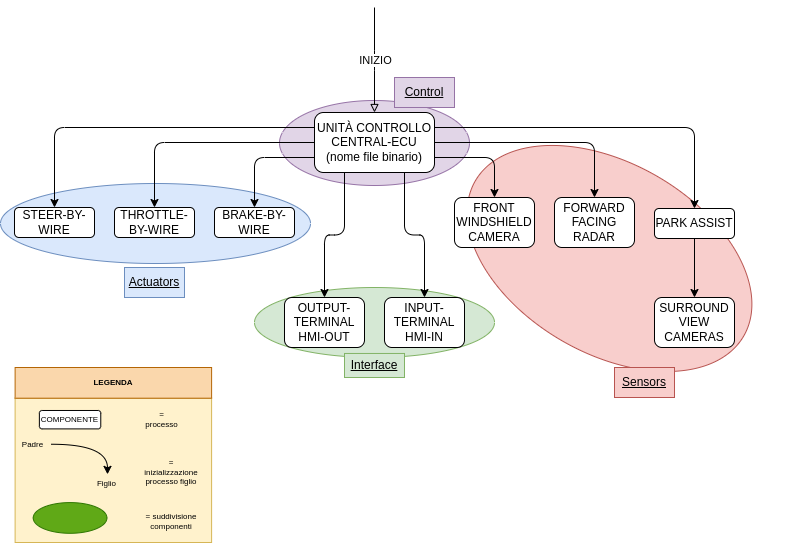
\includegraphics[scale=0.6, center]{./include/SO_Progetto_Diagrammi-Gerarchia.png}
				\caption{ In figura è mostrata la gerarchia implementata nel programma, nel quale la \textit{central-ECU} rappresenta il processo antenato di tutte gli altri processi.}
				\label{fig:gerarchia}
			\end{figure}



			\begin{figure}[h]
				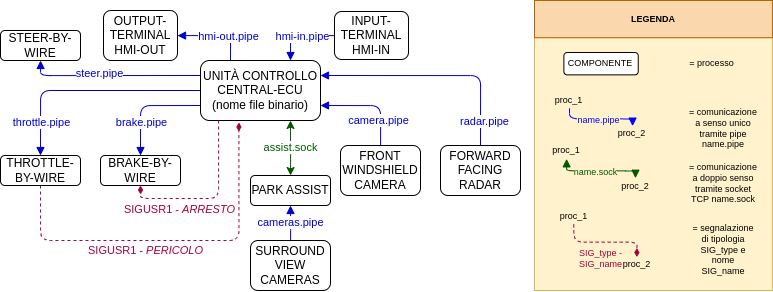
\includegraphics[scale=0.6, center]{./include/SO_Progetto_Diagrammi-Comunicazione.png}
				\caption{ In figura è mostrata la .}
				\label{fig:comunicazione}
			\end{figure}


			\newpage


	\newpage
	\hrule
	\tableofcontents

\end{document}